\section{Konzept}

Mithilfe der im vorherigen Kapitel erklärten Grundlagen können wir nun den konzeptionellen Aufbau der Glücksspielanwendung erklären.\newline
\newline

Der Ablauf des Spiels ist mit dem Ablauf aus dem Bitcoin Kapitels nahezu identisch. Die Unterschiede sind, dass 
enumerate\\
Das gesamte Spiel wird vom Benutzer initiiert.
\\
Der Gewinner wird anderes als bei Bitcoin nicht durch die letzte Zahl des Blockhashs, sondern durch den gesamten Wert des Blockhashes ermittelt. Hier dann angeben warum und auf das vorherige kapitel verweisen, dass erklärt, dass das so in ordung ist.
\\ TODO


\begin{figure}[H]
\centering
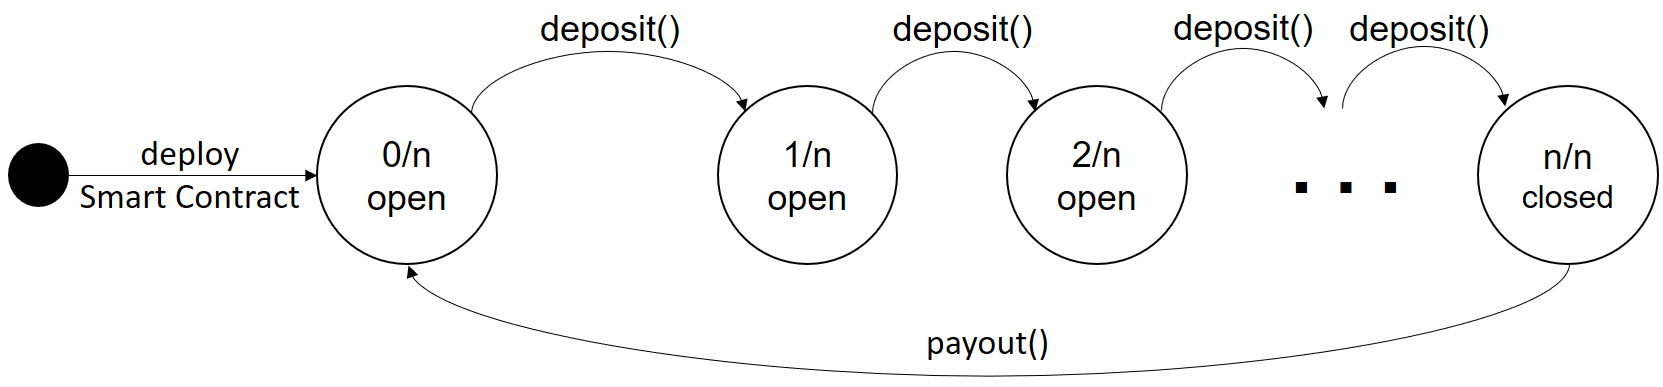
\includegraphics[width=1\linewidth]{Figures/umsetzung_eth/smart_contract_automat_idea}
\decoRule
\caption{Smart Contract Automat}
\label{fig:smart_contract_automat_idea}
\end{figure}

Der Blockhash der den Gewinner des Topfs entscheidet, muss in der Zukunft liegen und darf nicht vorher bekannt sein, da sonst Betrugsmöglichkeiten entstehen. Zum Zeitpunkt der letzten Einzahlungstransaktion ist es nicht möglich aus dem Smart Contract Code heraus auf den Blockhash des Blocks zuzugreifen in dem sich die letzte Einzahlungstransaktion befindet. Dies liegt daran, dass die Miner das Resultat der Zustandsveränderung aller Transaktionen des Blockes in den Blockheader schreiben müssen und erst anschließend den Blockhash berechnen. Die Transaktionen, die den Contract Code ausführen, können somit nicht auf den Blockhash zugreifen, da dieser zum Zeitpunkt der Codeausführung noch nicht feststeht. 

Bei Ethereum ist es also unumgänglich nach der letzten Einzahlungstransaktion eine Funktion aufzurufen, um den Gewinner auszuwählen und die Auszahlung zu starten.
Da der Smart Contract dies nicht selber kann, muss der Aufruf entweder von außerhalb oder von einem Anderen Smart Contract kommen.

a) Aufruf von außerhalb:\\
Der Aufruf kann wie in der Implementierung vom Gewinner ausgeführt werden. In diesem Fall zahlt der Gewinner die Transaktionsgebühr und erhält den gesamten Topf-Betrag. Der Gewinner ist dafür zuständig die Funktion rechtzeitig aufzurufen, da der Gewinn sonst in den nächsten Topf übergeht. Eine andere Möglichkeit ist es, dass die Glücksspielanwendung den Smart Contract überwacht und die \textit{payout} Funktion rechtzeitig aufruft. In diesem Fall müsste die Transaktionsgebühr von der Glücksspielanwendung gezahlt werden oder Funktionalität in den Smart Contract eingebaut werden, die die Transaktionskosten vom Topf-Betrag abzieht und der Glücksspielanwendung zurückerstattet. Allerdings verlässt sich der Gewinner dann auf die Anwendung und geht dadurch ein Risiko ein.

b) Aufruf durch Smart Contract:\\
Man kann in der Theorie den Ansatz des Ethereum Alarm Clock \footnote{\url{http://www.ethereum-alarm-clock.com/}} Contracts \footnote{\url{https://etherscan.io/address/0x6c8f2a135f6ed072de4503bd7c4999a1a17f824b}} verwenden, um eine gewünschte Smart Contract Funktion zu einem späteren Zeitpunkt auszuführen. Man spezifiziert dazu welche Funktion man wann (in welchem Blockzeitraum) ausführen möchte und zahlt für die anfallenden Transaktionsgebühren im Voraus. Dies erlaubt, dass eine ganze Reihe von Funktionen sich bei dem Alarm Clock Contract registrieren. Wird nun der Alarm Clock Contract von einem durch einen privaten Schlüssel kontrollierten Account ausgelöst, werden alle registrierten Funktionen aufgerufen. Leider liefert diese Vorgehensweise keine  Garantie, da eine registrierte Funktion nur aufgerufen wird, falls der Alarm Clock Contract aufgerufen wird. Die Glücksspielanwendung müsste also einspringen, sobald niemand anderes bereit ist den Alarm Clock Contract anzustoßen. Es handelt sich also lediglich um eine Vorgehensweise um Transaktionsgebühren mit anderen Ethereum Nutzern zu teilen.